\documentclass[11pt]{ctexart}

    \usepackage[breakable]{tcolorbox}
    \usepackage{parskip} % Stop auto-indenting (to mimic markdown behaviour)
    \usepackage{graphicx}
    \usepackage{float}
    \usepackage{iftex}
    \ifPDFTeX
    	\usepackage[T1]{fontenc}
    	\usepackage{mathpazo}
    \else
    	\usepackage{fontspec}
    \fi

    % Basic figure setup, for now with no caption control since it's done
    % automatically by Pandoc (which extracts ![](path) syntax from Markdown).
    \usepackage{graphicx}
    % Maintain compatibility with old templates. Remove in nbconvert 6.0
    \let\Oldincludegraphics\includegraphics
    % Ensure that by default, figures have no caption (until we provide a
    % proper Figure object with a Caption API and a way to capture that
    % in the conversion process - todo).
    \usepackage{caption}
    \DeclareCaptionFormat{nocaption}{}
    \captionsetup{format=nocaption,aboveskip=0pt,belowskip=0pt}

    \usepackage[Export]{adjustbox} % Used to constrain images to a maximum size
    \adjustboxset{max size={0.9\linewidth}{0.9\paperheight}}
    \usepackage{float}
    \floatplacement{figure}{H} % forces figures to be placed at the correct location
    \usepackage{xcolor} % Allow colors to be defined
    \usepackage{enumerate} % Needed for markdown enumerations to work
    \usepackage{geometry} % Used to adjust the document margins
    \usepackage{amsmath} % Equations
    \usepackage{amssymb} % Equations
    \usepackage{textcomp} % defines textquotesingle
    % Hack from http://tex.stackexchange.com/a/47451/13684:
    \AtBeginDocument{%
        \def\PYZsq{\textquotesingle}% Upright quotes in Pygmentized code
    }
    \usepackage{upquote} % Upright quotes for verbatim code
    \usepackage{eurosym} % defines \euro
    \usepackage[mathletters]{ucs} % Extended unicode (utf-8) support
    \usepackage{fancyvrb} % verbatim replacement that allows latex
    \usepackage{grffile} % extends the file name processing of package graphics 
                         % to support a larger range
    \makeatletter % fix for grffile with XeLaTeX
    \def\Gread@@xetex#1{%
      \IfFileExists{"\Gin@base".bb}%
      {\Gread@eps{\Gin@base.bb}}%
      {\Gread@@xetex@aux#1}%
    }
    \makeatother

    % The hyperref package gives us a pdf with properly built
    % internal navigation ('pdf bookmarks' for the table of contents,
    % internal cross-reference links, web links for URLs, etc.)
    \usepackage{hyperref}
    % The default LaTeX title has an obnoxious amount of whitespace. By default,
    % titling removes some of it. It also provides customization options.
    \usepackage{titling}
    \usepackage{longtable} % longtable support required by pandoc >1.10
    \usepackage{booktabs}  % table support for pandoc > 1.12.2
    \usepackage[inline]{enumitem} % IRkernel/repr support (it uses the enumerate* environment)
    \usepackage[normalem]{ulem} % ulem is needed to support strikethroughs (\sout)
                                % normalem makes italics be italics, not underlines
    \usepackage{mathrsfs}
    

    
    % Colors for the hyperref package
    \definecolor{urlcolor}{rgb}{0,.145,.698}
    \definecolor{linkcolor}{rgb}{.71,0.21,0.01}
    \definecolor{citecolor}{rgb}{.12,.54,.11}

    % ANSI colors
    \definecolor{ansi-black}{HTML}{3E424D}
    \definecolor{ansi-black-intense}{HTML}{282C36}
    \definecolor{ansi-red}{HTML}{E75C58}
    \definecolor{ansi-red-intense}{HTML}{B22B31}
    \definecolor{ansi-green}{HTML}{00A250}
    \definecolor{ansi-green-intense}{HTML}{007427}
    \definecolor{ansi-yellow}{HTML}{DDB62B}
    \definecolor{ansi-yellow-intense}{HTML}{B27D12}
    \definecolor{ansi-blue}{HTML}{208FFB}
    \definecolor{ansi-blue-intense}{HTML}{0065CA}
    \definecolor{ansi-magenta}{HTML}{D160C4}
    \definecolor{ansi-magenta-intense}{HTML}{A03196}
    \definecolor{ansi-cyan}{HTML}{60C6C8}
    \definecolor{ansi-cyan-intense}{HTML}{258F8F}
    \definecolor{ansi-white}{HTML}{C5C1B4}
    \definecolor{ansi-white-intense}{HTML}{A1A6B2}
    \definecolor{ansi-default-inverse-fg}{HTML}{FFFFFF}
    \definecolor{ansi-default-inverse-bg}{HTML}{000000}

    % commands and environments needed by pandoc snippets
    % extracted from the output of `pandoc -s`
    \providecommand{\tightlist}{%
      \setlength{\itemsep}{0pt}\setlength{\parskip}{0pt}}
    \DefineVerbatimEnvironment{Highlighting}{Verbatim}{commandchars=\\\{\}}
    % Add ',fontsize=\small' for more characters per line
    \newenvironment{Shaded}{}{}
    \newcommand{\KeywordTok}[1]{\textcolor[rgb]{0.00,0.44,0.13}{\textbf{{#1}}}}
    \newcommand{\DataTypeTok}[1]{\textcolor[rgb]{0.56,0.13,0.00}{{#1}}}
    \newcommand{\DecValTok}[1]{\textcolor[rgb]{0.25,0.63,0.44}{{#1}}}
    \newcommand{\BaseNTok}[1]{\textcolor[rgb]{0.25,0.63,0.44}{{#1}}}
    \newcommand{\FloatTok}[1]{\textcolor[rgb]{0.25,0.63,0.44}{{#1}}}
    \newcommand{\CharTok}[1]{\textcolor[rgb]{0.25,0.44,0.63}{{#1}}}
    \newcommand{\StringTok}[1]{\textcolor[rgb]{0.25,0.44,0.63}{{#1}}}
    \newcommand{\CommentTok}[1]{\textcolor[rgb]{0.38,0.63,0.69}{\textit{{#1}}}}
    \newcommand{\OtherTok}[1]{\textcolor[rgb]{0.00,0.44,0.13}{{#1}}}
    \newcommand{\AlertTok}[1]{\textcolor[rgb]{1.00,0.00,0.00}{\textbf{{#1}}}}
    \newcommand{\FunctionTok}[1]{\textcolor[rgb]{0.02,0.16,0.49}{{#1}}}
    \newcommand{\RegionMarkerTok}[1]{{#1}}
    \newcommand{\ErrorTok}[1]{\textcolor[rgb]{1.00,0.00,0.00}{\textbf{{#1}}}}
    \newcommand{\NormalTok}[1]{{#1}}
    
    % Additional commands for more recent versions of Pandoc
    \newcommand{\ConstantTok}[1]{\textcolor[rgb]{0.53,0.00,0.00}{{#1}}}
    \newcommand{\SpecialCharTok}[1]{\textcolor[rgb]{0.25,0.44,0.63}{{#1}}}
    \newcommand{\VerbatimStringTok}[1]{\textcolor[rgb]{0.25,0.44,0.63}{{#1}}}
    \newcommand{\SpecialStringTok}[1]{\textcolor[rgb]{0.73,0.40,0.53}{{#1}}}
    \newcommand{\ImportTok}[1]{{#1}}
    \newcommand{\DocumentationTok}[1]{\textcolor[rgb]{0.73,0.13,0.13}{\textit{{#1}}}}
    \newcommand{\AnnotationTok}[1]{\textcolor[rgb]{0.38,0.63,0.69}{\textbf{\textit{{#1}}}}}
    \newcommand{\CommentVarTok}[1]{\textcolor[rgb]{0.38,0.63,0.69}{\textbf{\textit{{#1}}}}}
    \newcommand{\VariableTok}[1]{\textcolor[rgb]{0.10,0.09,0.49}{{#1}}}
    \newcommand{\ControlFlowTok}[1]{\textcolor[rgb]{0.00,0.44,0.13}{\textbf{{#1}}}}
    \newcommand{\OperatorTok}[1]{\textcolor[rgb]{0.40,0.40,0.40}{{#1}}}
    \newcommand{\BuiltInTok}[1]{{#1}}
    \newcommand{\ExtensionTok}[1]{{#1}}
    \newcommand{\PreprocessorTok}[1]{\textcolor[rgb]{0.74,0.48,0.00}{{#1}}}
    \newcommand{\AttributeTok}[1]{\textcolor[rgb]{0.49,0.56,0.16}{{#1}}}
    \newcommand{\InformationTok}[1]{\textcolor[rgb]{0.38,0.63,0.69}{\textbf{\textit{{#1}}}}}
    \newcommand{\WarningTok}[1]{\textcolor[rgb]{0.38,0.63,0.69}{\textbf{\textit{{#1}}}}}
    
    
    % Define a nice break command that doesn't care if a line doesn't already
    % exist.
    \def\br{\hspace*{\fill} \\* }
    % Math Jax compatibility definitions
    \def\gt{>}
    \def\lt{<}
    \let\Oldtex\TeX
    \let\Oldlatex\LaTeX
    \renewcommand{\TeX}{\textrm{\Oldtex}}
    \renewcommand{\LaTeX}{\textrm{\Oldlatex}}
    % Document parameters
    % Document title
    \title{Unit67\_HW}
    
    
    
    
    
% Pygments definitions
\makeatletter
\def\PY@reset{\let\PY@it=\relax \let\PY@bf=\relax%
    \let\PY@ul=\relax \let\PY@tc=\relax%
    \let\PY@bc=\relax \let\PY@ff=\relax}
\def\PY@tok#1{\csname PY@tok@#1\endcsname}
\def\PY@toks#1+{\ifx\relax#1\empty\else%
    \PY@tok{#1}\expandafter\PY@toks\fi}
\def\PY@do#1{\PY@bc{\PY@tc{\PY@ul{%
    \PY@it{\PY@bf{\PY@ff{#1}}}}}}}
\def\PY#1#2{\PY@reset\PY@toks#1+\relax+\PY@do{#2}}

\expandafter\def\csname PY@tok@w\endcsname{\def\PY@tc##1{\textcolor[rgb]{0.73,0.73,0.73}{##1}}}
\expandafter\def\csname PY@tok@c\endcsname{\let\PY@it=\textit\def\PY@tc##1{\textcolor[rgb]{0.25,0.50,0.50}{##1}}}
\expandafter\def\csname PY@tok@cp\endcsname{\def\PY@tc##1{\textcolor[rgb]{0.74,0.48,0.00}{##1}}}
\expandafter\def\csname PY@tok@k\endcsname{\let\PY@bf=\textbf\def\PY@tc##1{\textcolor[rgb]{0.00,0.50,0.00}{##1}}}
\expandafter\def\csname PY@tok@kp\endcsname{\def\PY@tc##1{\textcolor[rgb]{0.00,0.50,0.00}{##1}}}
\expandafter\def\csname PY@tok@kt\endcsname{\def\PY@tc##1{\textcolor[rgb]{0.69,0.00,0.25}{##1}}}
\expandafter\def\csname PY@tok@o\endcsname{\def\PY@tc##1{\textcolor[rgb]{0.40,0.40,0.40}{##1}}}
\expandafter\def\csname PY@tok@ow\endcsname{\let\PY@bf=\textbf\def\PY@tc##1{\textcolor[rgb]{0.67,0.13,1.00}{##1}}}
\expandafter\def\csname PY@tok@nb\endcsname{\def\PY@tc##1{\textcolor[rgb]{0.00,0.50,0.00}{##1}}}
\expandafter\def\csname PY@tok@nf\endcsname{\def\PY@tc##1{\textcolor[rgb]{0.00,0.00,1.00}{##1}}}
\expandafter\def\csname PY@tok@nc\endcsname{\let\PY@bf=\textbf\def\PY@tc##1{\textcolor[rgb]{0.00,0.00,1.00}{##1}}}
\expandafter\def\csname PY@tok@nn\endcsname{\let\PY@bf=\textbf\def\PY@tc##1{\textcolor[rgb]{0.00,0.00,1.00}{##1}}}
\expandafter\def\csname PY@tok@ne\endcsname{\let\PY@bf=\textbf\def\PY@tc##1{\textcolor[rgb]{0.82,0.25,0.23}{##1}}}
\expandafter\def\csname PY@tok@nv\endcsname{\def\PY@tc##1{\textcolor[rgb]{0.10,0.09,0.49}{##1}}}
\expandafter\def\csname PY@tok@no\endcsname{\def\PY@tc##1{\textcolor[rgb]{0.53,0.00,0.00}{##1}}}
\expandafter\def\csname PY@tok@nl\endcsname{\def\PY@tc##1{\textcolor[rgb]{0.63,0.63,0.00}{##1}}}
\expandafter\def\csname PY@tok@ni\endcsname{\let\PY@bf=\textbf\def\PY@tc##1{\textcolor[rgb]{0.60,0.60,0.60}{##1}}}
\expandafter\def\csname PY@tok@na\endcsname{\def\PY@tc##1{\textcolor[rgb]{0.49,0.56,0.16}{##1}}}
\expandafter\def\csname PY@tok@nt\endcsname{\let\PY@bf=\textbf\def\PY@tc##1{\textcolor[rgb]{0.00,0.50,0.00}{##1}}}
\expandafter\def\csname PY@tok@nd\endcsname{\def\PY@tc##1{\textcolor[rgb]{0.67,0.13,1.00}{##1}}}
\expandafter\def\csname PY@tok@s\endcsname{\def\PY@tc##1{\textcolor[rgb]{0.73,0.13,0.13}{##1}}}
\expandafter\def\csname PY@tok@sd\endcsname{\let\PY@it=\textit\def\PY@tc##1{\textcolor[rgb]{0.73,0.13,0.13}{##1}}}
\expandafter\def\csname PY@tok@si\endcsname{\let\PY@bf=\textbf\def\PY@tc##1{\textcolor[rgb]{0.73,0.40,0.53}{##1}}}
\expandafter\def\csname PY@tok@se\endcsname{\let\PY@bf=\textbf\def\PY@tc##1{\textcolor[rgb]{0.73,0.40,0.13}{##1}}}
\expandafter\def\csname PY@tok@sr\endcsname{\def\PY@tc##1{\textcolor[rgb]{0.73,0.40,0.53}{##1}}}
\expandafter\def\csname PY@tok@ss\endcsname{\def\PY@tc##1{\textcolor[rgb]{0.10,0.09,0.49}{##1}}}
\expandafter\def\csname PY@tok@sx\endcsname{\def\PY@tc##1{\textcolor[rgb]{0.00,0.50,0.00}{##1}}}
\expandafter\def\csname PY@tok@m\endcsname{\def\PY@tc##1{\textcolor[rgb]{0.40,0.40,0.40}{##1}}}
\expandafter\def\csname PY@tok@gh\endcsname{\let\PY@bf=\textbf\def\PY@tc##1{\textcolor[rgb]{0.00,0.00,0.50}{##1}}}
\expandafter\def\csname PY@tok@gu\endcsname{\let\PY@bf=\textbf\def\PY@tc##1{\textcolor[rgb]{0.50,0.00,0.50}{##1}}}
\expandafter\def\csname PY@tok@gd\endcsname{\def\PY@tc##1{\textcolor[rgb]{0.63,0.00,0.00}{##1}}}
\expandafter\def\csname PY@tok@gi\endcsname{\def\PY@tc##1{\textcolor[rgb]{0.00,0.63,0.00}{##1}}}
\expandafter\def\csname PY@tok@gr\endcsname{\def\PY@tc##1{\textcolor[rgb]{1.00,0.00,0.00}{##1}}}
\expandafter\def\csname PY@tok@ge\endcsname{\let\PY@it=\textit}
\expandafter\def\csname PY@tok@gs\endcsname{\let\PY@bf=\textbf}
\expandafter\def\csname PY@tok@gp\endcsname{\let\PY@bf=\textbf\def\PY@tc##1{\textcolor[rgb]{0.00,0.00,0.50}{##1}}}
\expandafter\def\csname PY@tok@go\endcsname{\def\PY@tc##1{\textcolor[rgb]{0.53,0.53,0.53}{##1}}}
\expandafter\def\csname PY@tok@gt\endcsname{\def\PY@tc##1{\textcolor[rgb]{0.00,0.27,0.87}{##1}}}
\expandafter\def\csname PY@tok@err\endcsname{\def\PY@bc##1{\setlength{\fboxsep}{0pt}\fcolorbox[rgb]{1.00,0.00,0.00}{1,1,1}{\strut ##1}}}
\expandafter\def\csname PY@tok@kc\endcsname{\let\PY@bf=\textbf\def\PY@tc##1{\textcolor[rgb]{0.00,0.50,0.00}{##1}}}
\expandafter\def\csname PY@tok@kd\endcsname{\let\PY@bf=\textbf\def\PY@tc##1{\textcolor[rgb]{0.00,0.50,0.00}{##1}}}
\expandafter\def\csname PY@tok@kn\endcsname{\let\PY@bf=\textbf\def\PY@tc##1{\textcolor[rgb]{0.00,0.50,0.00}{##1}}}
\expandafter\def\csname PY@tok@kr\endcsname{\let\PY@bf=\textbf\def\PY@tc##1{\textcolor[rgb]{0.00,0.50,0.00}{##1}}}
\expandafter\def\csname PY@tok@bp\endcsname{\def\PY@tc##1{\textcolor[rgb]{0.00,0.50,0.00}{##1}}}
\expandafter\def\csname PY@tok@fm\endcsname{\def\PY@tc##1{\textcolor[rgb]{0.00,0.00,1.00}{##1}}}
\expandafter\def\csname PY@tok@vc\endcsname{\def\PY@tc##1{\textcolor[rgb]{0.10,0.09,0.49}{##1}}}
\expandafter\def\csname PY@tok@vg\endcsname{\def\PY@tc##1{\textcolor[rgb]{0.10,0.09,0.49}{##1}}}
\expandafter\def\csname PY@tok@vi\endcsname{\def\PY@tc##1{\textcolor[rgb]{0.10,0.09,0.49}{##1}}}
\expandafter\def\csname PY@tok@vm\endcsname{\def\PY@tc##1{\textcolor[rgb]{0.10,0.09,0.49}{##1}}}
\expandafter\def\csname PY@tok@sa\endcsname{\def\PY@tc##1{\textcolor[rgb]{0.73,0.13,0.13}{##1}}}
\expandafter\def\csname PY@tok@sb\endcsname{\def\PY@tc##1{\textcolor[rgb]{0.73,0.13,0.13}{##1}}}
\expandafter\def\csname PY@tok@sc\endcsname{\def\PY@tc##1{\textcolor[rgb]{0.73,0.13,0.13}{##1}}}
\expandafter\def\csname PY@tok@dl\endcsname{\def\PY@tc##1{\textcolor[rgb]{0.73,0.13,0.13}{##1}}}
\expandafter\def\csname PY@tok@s2\endcsname{\def\PY@tc##1{\textcolor[rgb]{0.73,0.13,0.13}{##1}}}
\expandafter\def\csname PY@tok@sh\endcsname{\def\PY@tc##1{\textcolor[rgb]{0.73,0.13,0.13}{##1}}}
\expandafter\def\csname PY@tok@s1\endcsname{\def\PY@tc##1{\textcolor[rgb]{0.73,0.13,0.13}{##1}}}
\expandafter\def\csname PY@tok@mb\endcsname{\def\PY@tc##1{\textcolor[rgb]{0.40,0.40,0.40}{##1}}}
\expandafter\def\csname PY@tok@mf\endcsname{\def\PY@tc##1{\textcolor[rgb]{0.40,0.40,0.40}{##1}}}
\expandafter\def\csname PY@tok@mh\endcsname{\def\PY@tc##1{\textcolor[rgb]{0.40,0.40,0.40}{##1}}}
\expandafter\def\csname PY@tok@mi\endcsname{\def\PY@tc##1{\textcolor[rgb]{0.40,0.40,0.40}{##1}}}
\expandafter\def\csname PY@tok@il\endcsname{\def\PY@tc##1{\textcolor[rgb]{0.40,0.40,0.40}{##1}}}
\expandafter\def\csname PY@tok@mo\endcsname{\def\PY@tc##1{\textcolor[rgb]{0.40,0.40,0.40}{##1}}}
\expandafter\def\csname PY@tok@ch\endcsname{\let\PY@it=\textit\def\PY@tc##1{\textcolor[rgb]{0.25,0.50,0.50}{##1}}}
\expandafter\def\csname PY@tok@cm\endcsname{\let\PY@it=\textit\def\PY@tc##1{\textcolor[rgb]{0.25,0.50,0.50}{##1}}}
\expandafter\def\csname PY@tok@cpf\endcsname{\let\PY@it=\textit\def\PY@tc##1{\textcolor[rgb]{0.25,0.50,0.50}{##1}}}
\expandafter\def\csname PY@tok@c1\endcsname{\let\PY@it=\textit\def\PY@tc##1{\textcolor[rgb]{0.25,0.50,0.50}{##1}}}
\expandafter\def\csname PY@tok@cs\endcsname{\let\PY@it=\textit\def\PY@tc##1{\textcolor[rgb]{0.25,0.50,0.50}{##1}}}

\def\PYZbs{\char`\\}
\def\PYZus{\char`\_}
\def\PYZob{\char`\{}
\def\PYZcb{\char`\}}
\def\PYZca{\char`\^}
\def\PYZam{\char`\&}
\def\PYZlt{\char`\<}
\def\PYZgt{\char`\>}
\def\PYZsh{\char`\#}
\def\PYZpc{\char`\%}
\def\PYZdl{\char`\$}
\def\PYZhy{\char`\-}
\def\PYZsq{\char`\'}
\def\PYZdq{\char`\"}
\def\PYZti{\char`\~}
% for compatibility with earlier versions
\def\PYZat{@}
\def\PYZlb{[}
\def\PYZrb{]}
\makeatother


    % For linebreaks inside Verbatim environment from package fancyvrb. 
    \makeatletter
        \newbox\Wrappedcontinuationbox 
        \newbox\Wrappedvisiblespacebox 
        \newcommand*\Wrappedvisiblespace {\textcolor{red}{\textvisiblespace}} 
        \newcommand*\Wrappedcontinuationsymbol {\textcolor{red}{\llap{\tiny$\m@th\hookrightarrow$}}} 
        \newcommand*\Wrappedcontinuationindent {3ex } 
        \newcommand*\Wrappedafterbreak {\kern\Wrappedcontinuationindent\copy\Wrappedcontinuationbox} 
        % Take advantage of the already applied Pygments mark-up to insert 
        % potential linebreaks for TeX processing. 
        %        {, <, #, %, $, ' and ": go to next line. 
        %        _, }, ^, &, >, - and ~: stay at end of broken line. 
        % Use of \textquotesingle for straight quote. 
        \newcommand*\Wrappedbreaksatspecials {% 
            \def\PYGZus{\discretionary{\char`\_}{\Wrappedafterbreak}{\char`\_}}% 
            \def\PYGZob{\discretionary{}{\Wrappedafterbreak\char`\{}{\char`\{}}% 
            \def\PYGZcb{\discretionary{\char`\}}{\Wrappedafterbreak}{\char`\}}}% 
            \def\PYGZca{\discretionary{\char`\^}{\Wrappedafterbreak}{\char`\^}}% 
            \def\PYGZam{\discretionary{\char`\&}{\Wrappedafterbreak}{\char`\&}}% 
            \def\PYGZlt{\discretionary{}{\Wrappedafterbreak\char`\<}{\char`\<}}% 
            \def\PYGZgt{\discretionary{\char`\>}{\Wrappedafterbreak}{\char`\>}}% 
            \def\PYGZsh{\discretionary{}{\Wrappedafterbreak\char`\#}{\char`\#}}% 
            \def\PYGZpc{\discretionary{}{\Wrappedafterbreak\char`\%}{\char`\%}}% 
            \def\PYGZdl{\discretionary{}{\Wrappedafterbreak\char`\$}{\char`\$}}% 
            \def\PYGZhy{\discretionary{\char`\-}{\Wrappedafterbreak}{\char`\-}}% 
            \def\PYGZsq{\discretionary{}{\Wrappedafterbreak\textquotesingle}{\textquotesingle}}% 
            \def\PYGZdq{\discretionary{}{\Wrappedafterbreak\char`\"}{\char`\"}}% 
            \def\PYGZti{\discretionary{\char`\~}{\Wrappedafterbreak}{\char`\~}}% 
        } 
        % Some characters . , ; ? ! / are not pygmentized. 
        % This macro makes them "active" and they will insert potential linebreaks 
        \newcommand*\Wrappedbreaksatpunct {% 
            \lccode`\~`\.\lowercase{\def~}{\discretionary{\hbox{\char`\.}}{\Wrappedafterbreak}{\hbox{\char`\.}}}% 
            \lccode`\~`\,\lowercase{\def~}{\discretionary{\hbox{\char`\,}}{\Wrappedafterbreak}{\hbox{\char`\,}}}% 
            \lccode`\~`\;\lowercase{\def~}{\discretionary{\hbox{\char`\;}}{\Wrappedafterbreak}{\hbox{\char`\;}}}% 
            \lccode`\~`\:\lowercase{\def~}{\discretionary{\hbox{\char`\:}}{\Wrappedafterbreak}{\hbox{\char`\:}}}% 
            \lccode`\~`\?\lowercase{\def~}{\discretionary{\hbox{\char`\?}}{\Wrappedafterbreak}{\hbox{\char`\?}}}% 
            \lccode`\~`\!\lowercase{\def~}{\discretionary{\hbox{\char`\!}}{\Wrappedafterbreak}{\hbox{\char`\!}}}% 
            \lccode`\~`\/\lowercase{\def~}{\discretionary{\hbox{\char`\/}}{\Wrappedafterbreak}{\hbox{\char`\/}}}% 
            \catcode`\.\active
            \catcode`\,\active 
            \catcode`\;\active
            \catcode`\:\active
            \catcode`\?\active
            \catcode`\!\active
            \catcode`\/\active 
            \lccode`\~`\~ 	
        }
    \makeatother

    \let\OriginalVerbatim=\Verbatim
    \makeatletter
    \renewcommand{\Verbatim}[1][1]{%
        %\parskip\z@skip
        \sbox\Wrappedcontinuationbox {\Wrappedcontinuationsymbol}%
        \sbox\Wrappedvisiblespacebox {\FV@SetupFont\Wrappedvisiblespace}%
        \def\FancyVerbFormatLine ##1{\hsize\linewidth
            \vtop{\raggedright\hyphenpenalty\z@\exhyphenpenalty\z@
                \doublehyphendemerits\z@\finalhyphendemerits\z@
                \strut ##1\strut}%
        }%
        % If the linebreak is at a space, the latter will be displayed as visible
        % space at end of first line, and a continuation symbol starts next line.
        % Stretch/shrink are however usually zero for typewriter font.
        \def\FV@Space {%
            \nobreak\hskip\z@ plus\fontdimen3\font minus\fontdimen4\font
            \discretionary{\copy\Wrappedvisiblespacebox}{\Wrappedafterbreak}
            {\kern\fontdimen2\font}%
        }%
        
        % Allow breaks at special characters using \PYG... macros.
        \Wrappedbreaksatspecials
        % Breaks at punctuation characters . , ; ? ! and / need catcode=\active 	
        \OriginalVerbatim[#1,codes*=\Wrappedbreaksatpunct]%
    }
    \makeatother

    % Exact colors from NB
    \definecolor{incolor}{HTML}{303F9F}
    \definecolor{outcolor}{HTML}{D84315}
    \definecolor{cellborder}{HTML}{CFCFCF}
    \definecolor{cellbackground}{HTML}{F7F7F7}
    
    % prompt
    \makeatletter
    \newcommand{\boxspacing}{\kern\kvtcb@left@rule\kern\kvtcb@boxsep}
    \makeatother
    \newcommand{\prompt}[4]{
        \ttfamily\llap{{\color{#2}[#3]:\hspace{3pt}#4}}\vspace{-\baselineskip}
    }
    

    
    % Prevent overflowing lines due to hard-to-break entities
    \sloppy 
    % Setup hyperref package
    \hypersetup{
      breaklinks=true,  % so long urls are correctly broken across lines
      colorlinks=true,
      urlcolor=urlcolor,
      linkcolor=linkcolor,
      citecolor=citecolor,
      }
    % Slightly bigger margins than the latex defaults
    
    \geometry{verbose,tmargin=1in,bmargin=1in,lmargin=1in,rmargin=1in}
    
    

\begin{document}

\maketitle




\hypertarget{unit6-7-hw}{%
    \section{Unit6-7 HW}\label{unit6-7-hw}}

\begin{tcolorbox}[breakable, size=fbox, boxrule=1pt, pad at break*=1mm,colback=cellbackground, colframe=cellborder]
    \prompt{In}{incolor}{2}{\boxspacing}
    \begin{Verbatim}[commandchars=\\\{\}]
        \PY{k+kn}{import} \PY{n+nn}{numpy} \PY{k}{as} \PY{n+nn}{np}
        \PY{k+kn}{import} \PY{n+nn}{matplotlib}\PY{n+nn}{.}\PY{n+nn}{pyplot} \PY{k}{as} \PY{n+nn}{plt}
        \PY{k+kn}{import} \PY{n+nn}{seaborn} \PY{k}{as} \PY{n+nn}{sns}
        \PY{k+kn}{import} \PY{n+nn}{astropy}
        \PY{n}{sns}\PY{o}{.}\PY{n}{set\PYZus{}style}\PY{p}{(}\PY{l+s+s1}{\PYZsq{}}\PY{l+s+s1}{darkgrid}\PY{l+s+s1}{\PYZsq{}}\PY{p}{)}
        \PY{k+kn}{import} \PY{n+nn}{scipy}\PY{n+nn}{.}\PY{n+nn}{stats} \PY{k}{as} \PY{n+nn}{stats}
        \PY{k+kn}{from} \PY{n+nn}{IPython}\PY{n+nn}{.}\PY{n+nn}{core}\PY{n+nn}{.}\PY{n+nn}{interactiveshell} \PY{k+kn}{import} \PY{n}{InteractiveShell}
        \PY{n}{InteractiveShell}\PY{o}{.}\PY{n}{ast\PYZus{}node\PYZus{}interactivity} \PY{o}{=} \PY{l+s+s1}{\PYZsq{}}\PY{l+s+s1}{all}\PY{l+s+s1}{\PYZsq{}}
    \end{Verbatim}
\end{tcolorbox}

\hypertarget{hw-u6-1}{%
    \subsection{HW-U6-1}\label{hw-u6-1}}

\hypertarget{a-compute-the-sample-mean-direction}{%
    \paragraph{(a) Compute the sample mean
        direction}\label{a-compute-the-sample-mean-direction}}

\begin{tcolorbox}[breakable, size=fbox, boxrule=1pt, pad at break*=1mm,colback=cellbackground, colframe=cellborder]
    \prompt{In}{incolor}{8}{\boxspacing}
    \begin{Verbatim}[commandchars=\\\{\}]
        \PY{n}{theta}\PY{o}{=}\PY{n}{np}\PY{o}{.}\PY{n}{array}\PY{p}{(}\PY{p}{[}\PY{l+m+mi}{0}\PY{p}{,}\PY{l+m+mi}{45}\PY{p}{,}\PY{l+m+mi}{90}\PY{p}{,}\PY{l+m+mi}{135}\PY{p}{,}\PY{l+m+mi}{180}\PY{p}{,}\PY{l+m+mi}{225}\PY{p}{]}\PY{p}{)}\PY{o}{*}\PY{n}{astropy}\PY{o}{.}\PY{n}{units}\PY{o}{.}\PY{n}{deg}
        \PY{n}{freq}\PY{o}{=}\PY{n}{np}\PY{o}{.}\PY{n}{array}\PY{p}{(}\PY{p}{[}\PY{l+m+mi}{2}\PY{p}{,}\PY{l+m+mi}{4}\PY{p}{,}\PY{l+m+mi}{3}\PY{p}{,}\PY{l+m+mi}{1}\PY{p}{,}\PY{l+m+mi}{1}\PY{p}{,}\PY{l+m+mi}{1}\PY{p}{]}\PY{p}{)}
        \PY{n}{theta}
        \PY{n}{freq}
        \PY{n}{astropy}\PY{o}{.}\PY{n}{stats}\PY{o}{.}\PY{n}{circmean}\PY{p}{(}\PY{n}{theta}\PY{p}{,}\PY{n}{weights}\PY{o}{=}\PY{n}{freq}\PY{p}{)}
    \end{Verbatim}
\end{tcolorbox}


\prompt{Out}{outcolor}{8}{}

$[0,~45,~90,~135,~180,~225] \; \mathrm{{}^{\circ}}$



\begin{tcolorbox}[breakable, size=fbox, boxrule=.5pt, pad at break*=1mm, opacityfill=0]
    \prompt{Out}{outcolor}{8}{\boxspacing}
    \begin{Verbatim}[commandchars=\\\{\}]
        array([2, 4, 3, 1, 1, 1])
    \end{Verbatim}
\end{tcolorbox}


\prompt{Out}{outcolor}{8}{}

$67.5 \; \mathrm{{}^{\circ}}$



方向的均值是67.5\(^\circ\)

\hypertarget{b-compute-the-angular-deviation-for-the-data}{%
    \paragraph{(b) Compute the angular deviation for the
        data}\label{b-compute-the-angular-deviation-for-the-data}}

\begin{tcolorbox}[breakable, size=fbox, boxrule=1pt, pad at break*=1mm,colback=cellbackground, colframe=cellborder]
    \prompt{In}{incolor}{15}{\boxspacing}
    \begin{Verbatim}[commandchars=\\\{\}]
        \PY{n}{n}\PY{o}{=}\PY{n+nb}{sum}\PY{p}{(}\PY{n}{freq}\PY{p}{)}
        \PY{n}{Y}\PY{o}{=}\PY{n+nb}{sum}\PY{p}{(}\PY{n}{freq}\PY{o}{*}\PY{n}{np}\PY{o}{.}\PY{n}{sin}\PY{p}{(}\PY{n}{theta}\PY{p}{)}\PY{p}{)}\PY{o}{/}\PY{n}{n}
        \PY{n}{X}\PY{o}{=}\PY{n+nb}{sum}\PY{p}{(}\PY{n}{freq}\PY{o}{*}\PY{n}{np}\PY{o}{.}\PY{n}{cos}\PY{p}{(}\PY{n}{theta}\PY{p}{)}\PY{p}{)}\PY{o}{/}\PY{n}{n}
        \PY{n}{r}\PY{o}{=}\PY{n}{np}\PY{o}{.}\PY{n}{sqrt}\PY{p}{(}\PY{n}{X}\PY{o}{*}\PY{o}{*}\PY{l+m+mi}{2}\PY{o}{+}\PY{n}{Y}\PY{o}{*}\PY{o}{*}\PY{l+m+mi}{2}\PY{p}{)}
        \PY{n}{r}
        \PY{l+m+mi}{1}\PY{o}{\PYZhy{}}\PY{n}{r}
        \PY{l+m+mi}{2}\PY{o}{*}\PY{p}{(}\PY{l+m+mi}{1}\PY{o}{\PYZhy{}}\PY{n}{r}\PY{p}{)}
        \PY{n}{np}\PY{o}{.}\PY{n}{log}\PY{p}{(}\PY{l+m+mi}{1}\PY{o}{\PYZhy{}}\PY{n}{r}\PY{p}{)}
    \end{Verbatim}
\end{tcolorbox}


\prompt{Out}{outcolor}{15}{}

$0.52572034 \; \mathrm{}$




\prompt{Out}{outcolor}{15}{}

$0.47427966 \; \mathrm{}$




\prompt{Out}{outcolor}{15}{}

$0.94855932 \; \mathrm{}$




\prompt{Out}{outcolor}{15}{}

$-0.74595813 \; \mathrm{}$



\hypertarget{c-determine-95-confidence-limits-for-the-population-mean}{%
    \paragraph{(c) Determine 95\% confidence limits for the population
        mean}\label{c-determine-95-confidence-limits-for-the-population-mean}}

\begin{tcolorbox}[breakable, size=fbox, boxrule=1pt, pad at break*=1mm,colback=cellbackground, colframe=cellborder]
    \prompt{In}{incolor}{19}{\boxspacing}
    \begin{Verbatim}[commandchars=\\\{\}]
        \PY{k}{def} \PY{n+nf}{meand\PYZus{}ci}\PY{p}{(}\PY{n}{r}\PY{p}{,}\PY{n}{n}\PY{p}{,}\PY{n}{alpha}\PY{p}{)}\PY{p}{:}
        \PY{n}{R}\PY{o}{=}\PY{n}{r}\PY{o}{*}\PY{n}{n}
        \PY{n}{chi2}\PY{o}{=}\PY{n}{stats}\PY{o}{.}\PY{n}{chi2}\PY{o}{.}\PY{n}{isf}\PY{p}{(}\PY{n}{alpha}\PY{p}{,} \PY{l+m+mi}{1}\PY{p}{,} \PY{n}{loc}\PY{o}{=}\PY{l+m+mi}{0}\PY{p}{,} \PY{n}{scale}\PY{o}{=}\PY{l+m+mi}{1}\PY{p}{)}
        \PY{k}{if} \PY{n}{r}\PY{o}{\PYZgt{}}\PY{o}{=}\PY{l+m+mf}{0.9}\PY{p}{:}
        \PY{k}{return} \PY{n}{np}\PY{o}{.}\PY{n}{arccos}\PY{p}{(}\PY{n}{np}\PY{o}{.}\PY{n}{sqrt}\PY{p}{(}\PY{n}{n}\PY{o}{*}\PY{o}{*}\PY{l+m+mi}{2}\PY{o}{\PYZhy{}}\PY{p}{(}\PY{n}{n}\PY{o}{*}\PY{o}{*}\PY{l+m+mi}{2}\PY{o}{\PYZhy{}}\PY{n}{R}\PY{o}{*}\PY{o}{*}\PY{l+m+mi}{2}\PY{p}{)}\PY{o}{*}\PY{n}{np}\PY{o}{.}\PY{n}{e}\PY{o}{*}\PY{o}{*}\PY{p}{(}\PY{n}{chi2}\PY{o}{/}\PY{n}{n}\PY{p}{)}\PY{p}{)}\PY{o}{/}\PY{n}{R}\PY{p}{)}
        \PY{k}{else}\PY{p}{:}
        \PY{k}{return} \PY{n}{np}\PY{o}{.}\PY{n}{arccos}\PY{p}{(}\PY{n}{np}\PY{o}{.}\PY{n}{sqrt}\PY{p}{(}\PY{l+m+mi}{2}\PY{o}{*}\PY{n}{n}\PY{o}{*}\PY{p}{(}\PY{l+m+mi}{2}\PY{o}{*}\PY{n}{R}\PY{o}{*}\PY{o}{*}\PY{l+m+mi}{2}\PY{o}{\PYZhy{}}\PY{n}{n}\PY{o}{*}\PY{n}{chi2}\PY{p}{)}\PY{o}{/}\PY{p}{(}\PY{l+m+mi}{4}\PY{o}{*}\PY{n}{n}\PY{o}{\PYZhy{}}\PY{n}{chi2}\PY{p}{)}\PY{p}{)}\PY{o}{/}\PY{n}{R}\PY{p}{)}
    \end{Verbatim}
\end{tcolorbox}

\begin{tcolorbox}[breakable, size=fbox, boxrule=1pt, pad at break*=1mm,colback=cellbackground, colframe=cellborder]
    \prompt{In}{incolor}{31}{\boxspacing}
    \begin{Verbatim}[commandchars=\\\{\}]
        \PY{n}{data\PYZus{}mean}\PY{o}{=}\PY{n}{astropy}\PY{o}{.}\PY{n}{stats}\PY{o}{.}\PY{n}{circmean}\PY{p}{(}\PY{n}{theta}\PY{p}{,}\PY{n}{weights}\PY{o}{=}\PY{n}{freq}\PY{p}{)}
        \PY{n}{ci}\PY{o}{=}\PY{p}{(}\PY{n}{data\PYZus{}mean}\PY{o}{\PYZhy{}}\PY{n}{meand\PYZus{}ci}\PY{p}{(}\PY{n}{r}\PY{p}{,}\PY{n}{n}\PY{p}{,}\PY{l+m+mf}{0.05}\PY{p}{)}\PY{p}{,}\PY{n}{data\PYZus{}mean}\PY{o}{+}\PY{n}{meand\PYZus{}ci}\PY{p}{(}\PY{n}{r}\PY{p}{,}\PY{n}{n}\PY{p}{,}\PY{l+m+mf}{0.05}\PY{p}{)}\PY{p}{)}
        \PY{n}{ci}
    \end{Verbatim}
\end{tcolorbox}

\begin{tcolorbox}[breakable, size=fbox, boxrule=.5pt, pad at break*=1mm, opacityfill=0]
    \prompt{Out}{outcolor}{31}{\boxspacing}
    \begin{Verbatim}[commandchars=\\\{\}]
        12
    \end{Verbatim}
\end{tcolorbox}

\begin{tcolorbox}[breakable, size=fbox, boxrule=.5pt, pad at break*=1mm, opacityfill=0]
    \prompt{Out}{outcolor}{31}{\boxspacing}
    \begin{Verbatim}[commandchars=\\\{\}]
        (<Quantity 20.06103815 deg>, <Quantity 114.93896185 deg>)
    \end{Verbatim}
\end{tcolorbox}

均值的95\%置信区间是(20.06\(^\circ\),114.94\(^\circ\))

\hypertarget{d-determine-the-sample-median-direction}{%
    \paragraph{(d) Determine the sample median
        direction}\label{d-determine-the-sample-median-direction}}

\begin{tcolorbox}[breakable, size=fbox, boxrule=1pt, pad at break*=1mm,colback=cellbackground, colframe=cellborder]
    \prompt{In}{incolor}{32}{\boxspacing}
    \begin{Verbatim}[commandchars=\\\{\}]
        \PY{k}{def} \PY{n+nf}{sample\PYZus{}median}\PY{p}{(}\PY{n}{theta}\PY{p}{,}\PY{n}{freq}\PY{p}{)}\PY{p}{:}
        \PY{n}{n}\PY{o}{=}\PY{n+nb}{sum}\PY{p}{(}\PY{n}{freq}\PY{p}{)}
        \PY{n}{tmp}\PY{o}{=}\PY{n}{np}\PY{o}{.}\PY{n}{cumsum}\PY{p}{(}\PY{n}{freq}\PY{p}{)}
        \PY{k}{if} \PY{n}{n}\PY{o}{\PYZpc{}}\PY{k}{2}:
        \PY{k}{for} \PY{n}{i} \PY{o+ow}{in} \PY{n+nb}{range}\PY{p}{(}\PY{n+nb}{len}\PY{p}{(}\PY{n}{tmp}\PY{p}{)}\PY{p}{)}\PY{p}{:}
        \PY{k}{if} \PY{n}{tmp}\PY{p}{[}\PY{n}{i}\PY{p}{]}\PY{o}{\PYZgt{}}\PY{o}{=}\PY{p}{(}\PY{n}{n}\PY{o}{\PYZhy{}}\PY{l+m+mi}{1}\PY{p}{)}\PY{o}{/}\PY{l+m+mi}{2}\PY{p}{:}
        \PY{k}{break}
        \PY{k}{return} \PY{n}{theta}\PY{p}{[}\PY{n}{i}\PY{p}{]}
        \PY{k}{else} \PY{p}{:}
        \PY{k}{for} \PY{n}{i} \PY{o+ow}{in} \PY{n+nb}{range}\PY{p}{(}\PY{n+nb}{len}\PY{p}{(}\PY{n}{tmp}\PY{p}{)}\PY{p}{)}\PY{p}{:}
        \PY{k}{if} \PY{n}{tmp}\PY{p}{[}\PY{n}{i}\PY{p}{]}\PY{o}{\PYZgt{}}\PY{o}{=}\PY{n}{n}\PY{o}{/}\PY{l+m+mi}{2}\PY{o}{\PYZhy{}}\PY{l+m+mi}{1}\PY{p}{:}
        \PY{k}{break}
        \PY{n}{left}\PY{o}{=}\PY{n}{i}
        \PY{k}{for} \PY{n}{i} \PY{o+ow}{in} \PY{n+nb}{range}\PY{p}{(}\PY{n+nb}{len}\PY{p}{(}\PY{n}{tmp}\PY{p}{)}\PY{p}{)}\PY{p}{:}
        \PY{k}{if} \PY{n}{tmp}\PY{p}{[}\PY{n}{i}\PY{p}{]}\PY{o}{\PYZgt{}}\PY{o}{=}\PY{n}{n}\PY{o}{/}\PY{l+m+mi}{2}\PY{o}{+}\PY{l+m+mi}{1}\PY{p}{:}
        \PY{k}{break}
        \PY{n}{right}\PY{o}{=}\PY{n}{i}
        \PY{k}{return} \PY{p}{(}\PY{n}{theta}\PY{p}{[}\PY{n}{left}\PY{p}{]}\PY{o}{+}\PY{n}{theta}\PY{p}{[}\PY{n}{right}\PY{p}{]}\PY{p}{)}\PY{o}{/}\PY{l+m+mi}{2}
    \end{Verbatim}
\end{tcolorbox}

\begin{tcolorbox}[breakable, size=fbox, boxrule=1pt, pad at break*=1mm,colback=cellbackground, colframe=cellborder]
    \prompt{In}{incolor}{33}{\boxspacing}
    \begin{Verbatim}[commandchars=\\\{\}]
        \PY{n}{sample\PYZus{}median}\PY{p}{(}\PY{n}{theta}\PY{p}{,}\PY{n}{freq}\PY{p}{)}
    \end{Verbatim}
\end{tcolorbox}


\prompt{Out}{outcolor}{33}{}

$67.5 \; \mathrm{{}^{\circ}}$



\hypertarget{hw-u6-2}{%
    \subsection{HW-U6-2}\label{hw-u6-2}}

\hypertarget{visualize-the-data-in-problem-hw-6-1-in-polar-coodinates}{%
    \paragraph{Visualize the data in Problem HW-6-1 in polar
        coodinates}\label{visualize-the-data-in-problem-hw-6-1-in-polar-coodinates}}

\begin{tcolorbox}[breakable, size=fbox, boxrule=1pt, pad at break*=1mm,colback=cellbackground, colframe=cellborder]
    \prompt{In}{incolor}{65}{\boxspacing}
    \begin{Verbatim}[commandchars=\\\{\}]
        \PY{n}{width}\PY{o}{=}\PY{l+m+mf}{0.5}
        \PY{n}{data}\PY{o}{=}\PY{n}{np}\PY{o}{.}\PY{n}{array}\PY{p}{(}\PY{p}{[}\PY{l+m+mi}{0}\PY{p}{,}\PY{l+m+mi}{45}\PY{p}{,}\PY{l+m+mi}{90}\PY{p}{,}\PY{l+m+mi}{135}\PY{p}{,}\PY{l+m+mi}{180}\PY{p}{,}\PY{l+m+mi}{225}\PY{p}{]}\PY{p}{)}
        \PY{n}{ax} \PY{o}{=} \PY{n}{plt}\PY{o}{.}\PY{n}{subplot}\PY{p}{(}\PY{l+m+mi}{111}\PY{p}{,} \PY{n}{projection}\PY{o}{=}\PY{l+s+s1}{\PYZsq{}}\PY{l+s+s1}{polar}\PY{l+s+s1}{\PYZsq{}}\PY{p}{)}
        \PY{n}{ax}\PY{o}{.}\PY{n}{bar}\PY{p}{(}\PY{n}{data}\PY{p}{,} \PY{n}{freq}\PY{p}{,} \PY{n}{width}\PY{o}{=}\PY{n}{width}\PY{p}{,} \PY{n}{bottom}\PY{o}{=}\PY{l+m+mf}{0.0}\PY{p}{,} \PY{n}{alpha}\PY{o}{=}\PY{l+m+mf}{0.5}\PY{p}{)}
        \PY{n}{ax}\PY{o}{.}\PY{n}{scatter}\PY{p}{(}\PY{n}{data}\PY{p}{,}\PY{l+m+mf}{4.5}\PY{o}{*}\PY{n}{np}\PY{o}{.}\PY{n}{ones}\PY{p}{(}\PY{n+nb}{len}\PY{p}{(}\PY{n}{theta}\PY{p}{)}\PY{p}{)}\PY{p}{,}\PY{n}{marker}\PY{o}{=}\PY{l+s+s1}{\PYZsq{}}\PY{l+s+s1}{o}\PY{l+s+s1}{\PYZsq{}}\PY{p}{,} \PY{n}{s}\PY{o}{=}\PY{l+m+mi}{50}\PY{o}{*}\PY{n}{freq}\PY{p}{,}\PY{n}{alpha}\PY{o}{=}\PY{l+m+mf}{0.75}\PY{p}{)}
        \PY{n}{ax}\PY{o}{.}\PY{n}{tick\PYZus{}params}\PY{p}{(}\PY{n}{colors}\PY{o}{=}\PY{l+s+s1}{\PYZsq{}}\PY{l+s+s1}{red}\PY{l+s+s1}{\PYZsq{}}\PY{p}{)}
        \PY{n}{ax}\PY{o}{.}\PY{n}{set\PYZus{}rlim}\PY{p}{(}\PY{l+m+mi}{0}\PY{p}{,}\PY{l+m+mi}{5}\PY{p}{)}
        \PY{n}{plt}\PY{o}{.}\PY{n}{show}\PY{p}{(}\PY{p}{)}
    \end{Verbatim}
\end{tcolorbox}

\begin{tcolorbox}[breakable, size=fbox, boxrule=.5pt, pad at break*=1mm, opacityfill=0]
    \prompt{Out}{outcolor}{65}{\boxspacing}
    \begin{Verbatim}[commandchars=\\\{\}]
        <BarContainer object of 6 artists>
    \end{Verbatim}
\end{tcolorbox}

\begin{tcolorbox}[breakable, size=fbox, boxrule=.5pt, pad at break*=1mm, opacityfill=0]
    \prompt{Out}{outcolor}{65}{\boxspacing}
    \begin{Verbatim}[commandchars=\\\{\}]
        <matplotlib.collections.PathCollection at 0x1aa4609a9c8>
    \end{Verbatim}
\end{tcolorbox}

\begin{tcolorbox}[breakable, size=fbox, boxrule=.5pt, pad at break*=1mm, opacityfill=0]
    \prompt{Out}{outcolor}{65}{\boxspacing}
    \begin{Verbatim}[commandchars=\\\{\}]
        (0, 5)
    \end{Verbatim}
\end{tcolorbox}

\begin{center}
    \adjustimage{max size={0.9\linewidth}{0.9\paperheight}}{output_15_3.png}
\end{center}
{ \hspace*{\fill} \\}

\hypertarget{hw-u7-1}{%
    \subsection{HW-U7-1}\label{hw-u7-1}}

\hypertarget{ux5982ux679cux5728ux67d0ux4e00ux4e2aux5730ux533acovid-19ux7684ux611fux67d3ux7387ux572810ux4eceux8be5ux5730ux533aux4ebaux53e3ux4e2dux968fux673aux53d6ux6837nux4e2aux6837ux672cux8fdbux884cux5b9eux9a8cux7814ux7a76ux8981ux4f7fux5f97ux6837ux672cux611fux67d3ux7387ux8befux5deeux57285ux4ee5ux5185-95-confidence-levelnux81f3ux5c11ux5e94ux8be5ux8981ux91c7ux6837ux591aux5c11}{%
    \paragraph{如果在某一个地区covid-19的感染率在10\%,从该地区人口中随机取样N个样本进行实验研究,要使得样本感染率误差在5\%以内
        (95\% confidence
        level),N至少应该要采样多少?}\label{ux5982ux679cux5728ux67d0ux4e00ux4e2aux5730ux533acovid-19ux7684ux611fux67d3ux7387ux572810ux4eceux8be5ux5730ux533aux4ebaux53e3ux4e2dux968fux673aux53d6ux6837nux4e2aux6837ux672cux8fdbux884cux5b9eux9a8cux7814ux7a76ux8981ux4f7fux5f97ux6837ux672cux611fux67d3ux7387ux8befux5deeux57285ux4ee5ux5185-95-confidence-levelnux81f3ux5c11ux5e94ux8be5ux8981ux91c7ux6837ux591aux5c11}}

\begin{tcolorbox}[breakable, size=fbox, boxrule=1pt, pad at break*=1mm,colback=cellbackground, colframe=cellborder]
    \prompt{In}{incolor}{66}{\boxspacing}
    \begin{Verbatim}[commandchars=\\\{\}]
        \PY{k}{def} \PY{n+nf}{qualitative\PYZus{}n}\PY{p}{(}\PY{n}{z}\PY{p}{,}\PY{n}{p}\PY{p}{,}\PY{n}{d}\PY{p}{)}\PY{p}{:}
        \PY{k}{return} \PY{n}{z}\PY{o}{*}\PY{o}{*}\PY{l+m+mi}{2}\PY{o}{*}\PY{n}{p}\PY{o}{*}\PY{p}{(}\PY{l+m+mi}{1}\PY{o}{\PYZhy{}}\PY{n}{p}\PY{p}{)}\PY{o}{/}\PY{n}{d}\PY{o}{*}\PY{o}{*}\PY{l+m+mi}{2}
    \end{Verbatim}
\end{tcolorbox}

\begin{tcolorbox}[breakable, size=fbox, boxrule=1pt, pad at break*=1mm,colback=cellbackground, colframe=cellborder]
    \prompt{In}{incolor}{67}{\boxspacing}
    \begin{Verbatim}[commandchars=\\\{\}]
        \PY{n}{qualitative\PYZus{}n}\PY{p}{(}\PY{l+m+mi}{2}\PY{p}{,}\PY{l+m+mf}{0.1}\PY{p}{,}\PY{l+m+mf}{0.05}\PY{p}{)}
    \end{Verbatim}
\end{tcolorbox}

\begin{tcolorbox}[breakable, size=fbox, boxrule=.5pt, pad at break*=1mm, opacityfill=0]
    \prompt{Out}{outcolor}{67}{\boxspacing}
    \begin{Verbatim}[commandchars=\\\{\}]
        144.0
    \end{Verbatim}
\end{tcolorbox}

N至少要采样144。

\hypertarget{hw-u7-2}{%
    \subsection{HW-U7-2}\label{hw-u7-2}}

\hypertarget{ux5982ux679cux7a7aux8179ux8840ux7cd6ux5e73ux5747ux6c34ux5e73ux572890-mgdlux521dux6b65ux5b9eux9a8cux8868ux660eux67d0ux79cdux996eux6599ux5728ux534aux5c0fux65f6ux5185ux4f1aux63d0ux9ad8ux8840ux7cd6-3-mgdlux5047ux8bbeux8840ux7cd6ux7684ux6807ux51c6ux5deeux572810-mgdl-ux7814ux7a76ux540cux4e00ux6279ux4ebaux559dux996eux6599ux524dux540eux7684ux8840ux7cd6ux6c34ux5e73ux589eux52a0ux91cfux91c7ux7528paired--tux68c0ux9a8cux8981ux6c42nhstux663eux8457ux6c34ux5e73ux8fbeux523099ux7edfux8ba1powerux8fbeux52300.9-ux4f30ux7b97ux9700ux8981ux591aux5c11ux5927ux7684ux6837ux672cux91cf}{%
    \paragraph{如果空腹血糖平均水平在90
        mg/dl,初步实验表明某种饮料在半小时内会提高血糖 3
        mg/dl;假设血糖的标准差在10 mg/dl;
        研究同一批人喝饮料前后的血糖水平增加量,采用paired
        -t检验,要求NHST显著水平达到99\%,统计Power达到0.9
        ,估算需要多少大的样本量?}\label{ux5982ux679cux7a7aux8179ux8840ux7cd6ux5e73ux5747ux6c34ux5e73ux572890-mgdlux521dux6b65ux5b9eux9a8cux8868ux660eux67d0ux79cdux996eux6599ux5728ux534aux5c0fux65f6ux5185ux4f1aux63d0ux9ad8ux8840ux7cd6-3-mgdlux5047ux8bbeux8840ux7cd6ux7684ux6807ux51c6ux5deeux572810-mgdl-ux7814ux7a76ux540cux4e00ux6279ux4ebaux559dux996eux6599ux524dux540eux7684ux8840ux7cd6ux6c34ux5e73ux589eux52a0ux91cfux91c7ux7528paired--tux68c0ux9a8cux8981ux6c42nhstux663eux8457ux6c34ux5e73ux8fbeux523099ux7edfux8ba1powerux8fbeux52300.9-ux4f30ux7b97ux9700ux8981ux591aux5c11ux5927ux7684ux6837ux672cux91cf}}

\begin{figure}[H]
    \centering
    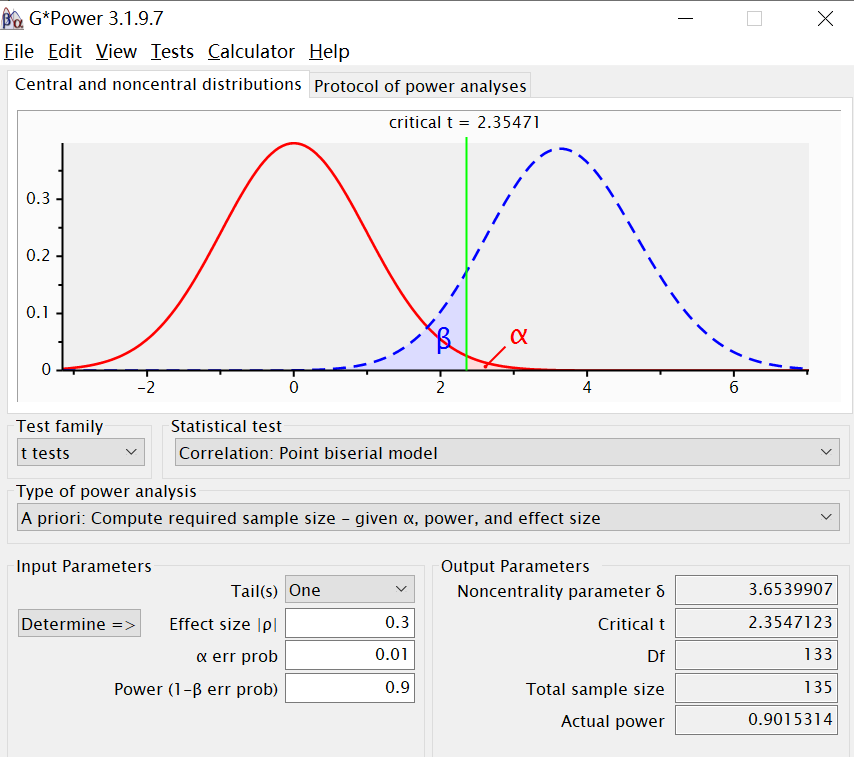
\includegraphics[width=0.7\textwidth]{7-2.png}
\end{figure}


根据G-Power的计算结果可知,需要样本量为135



\begin{tcolorbox}[breakable, size=fbox, boxrule=1pt, pad at break*=1mm,colback=cellbackground, colframe=cellborder]
    \prompt{In}{incolor}{ }{\boxspacing}
    \begin{Verbatim}[commandchars=\\\{\}]

    \end{Verbatim}
\end{tcolorbox}


% Add a bibliography block to the postdoc



\end{document}
